\documentclass[11pt,a4paper,dvipsnames]{article}
\usepackage[deliverable]{IOHKCoverPage}


\usepackage[margin=2.5cm]{geometry}
\usepackage{iohk}
\usepackage{microtype}
\usepackage{mathpazo} % nice fonts
\usepackage{amsmath}
\usepackage{amssymb}
\usepackage{amsthm}
\usepackage{latexsym}
\usepackage{mathtools}
\usepackage{stmaryrd}
\usepackage{extarrows}
\usepackage{slashed}
\usepackage[colon]{natbib}
\usepackage[unicode=true,pdftex,pdfa,colorlinks=true]{hyperref}
\usepackage{xcolor}
\usepackage[capitalise,noabbrev,nameinlink]{cleveref}
\usepackage{float}
\floatstyle{boxed}
\restylefloat{figure}
\usepackage{tikz}
\usepackage{booktabs}
\usepackage{enumerate}
\usepackage{comments} \newcommand{\khcomment}[1]{\comment{KH}{#1}}

\setlength{\parindent}{0pt}


%%
%% Package `semantic` can be used for writing inference rules.
%%
\usepackage{semantic}
%% Setup for the semantic package
\setpremisesspace{20pt}

% data for Deliverable header -- added by KH from an EU H2020 project template
\DeliverableNumber{VL-D1}
\DeliverableTitle{The Design of the Cardano Ledger with Automated Parameter Updates and Central Fund Transfers}{Design Document: Automated Updates/Fund Transfers}
\DeliverableResponsible{Formal Methods Team}
\EditorName{Andre Knispel, \IOHK}
\Authors{
   Andre Knispel \quad \texttt{andre.knispel@iohk.io}\\
   Kevin Hammond \quad \texttt{kevin.hammond@iohk.io}\\
   Philipp Kant \quad \texttt{philipp.kant@iohk.io}
   % TOOO: Order by main author:  KH
}
\DueDate{30$^{\textrm{th}}$ April 2021}
\SubmissionDate{}{}
\LeaderName{Philipp Kant, \IOHK}
\InstitutionAddress{\IOHK}
\Version{FS-5.0.0}
\Project{Voltaire Ledger}
\DisseminationDR

%%
%% Types
%%
\newcommand{\Nothing}{\ensuremath{\Diamond}}
\newcommand{\N}{\ensuremath{\mathbb{N}}}
\newcommand{\Bool}{\type{Bool}}
\newcommand{\Npos}{\ensuremath{\mathbb{N}^{+}}}
\newcommand{\Z}{\ensuremath{\mathbb{Z}}}
\newcommand{\R}{\ensuremath{\mathbb{R}}}
\newcommand{\Rnn}{\ensuremath{\mathbb{R}^{\geq 0}}}
\newcommand{\Tx}{\type{Tx}}
\newcommand{\ShelleyTx}{\type{ShelleyTx}}
\newcommand{\GoguenTx}{\type{GoguenTx}}
\newcommand{\TxBody}{\type{TxBody}}
\newcommand{\UnsignedData}{\type{UnsignedData}}
\newcommand{\VldSR}{\type{VldSR}}
\newcommand{\VldOut}{\type{VldOut}}
\newcommand{\Vlds}{\type{Vlds}}
\newcommand{\TxWitness}{\type{TxWitness}}
\newcommand{\Ix}{\type{Ix}}
\newcommand{\RdmrPtr}{\type{RdmrPtr}}
\newcommand{\TxId}{\type{TxId}}
\newcommand{\Addr}{\type{Addr}}
\newcommand{\UTxO}{\type{UTxO}}
\newcommand{\UTxOIn}{\type{UTxOIn}}
\newcommand{\Wdrl}{\type{Wdrl}}
\newcommand{\Coin}{\type{Coin}}
\newcommand{\PParams}{\type{PParams}}
\newcommand{\ShelleyPParams}{\type{ShelleyPParams}}
\newcommand{\NewParams}{\type{NewParams}}
\newcommand{\Slot}{\type{Slot}}
\newcommand{\SlotsPrior}{\ensuremath{\mathsf{SlotsPrior}}}
\newcommand{\SlotsPerEpoch}{\mathsf{SlotsPerEpoch}}
\newcommand{\SlotsPerKESPeriod}{\mathsf{SlotsPerKESPeriod}}
\newcommand{\SlotsStabilityParam}{\fun{k}}
\newcommand{\Duration}{\type{Duration}}
\newcommand{\StakePools}{\type{StakePools}}
\newcommand{\StakeDeleg}{\type{StakeDeleg}}
\newcommand{\StakeCreds}{\type{StakeCreds}}
\newcommand{\Seed}{\type{Seed}}
\newcommand{\seedOp}{\star}
\newcommand{\Ppm}{\type{Ppm}}
\newcommand{\Value}{\type{Value}}
\newcommand{\ProtVer}{\ensuremath{\type{ProtVer}}}
\newcommand{\Language}{\type{Language}}
\newcommand{\ApName}{\ensuremath{\type{ApName}}}
\newcommand{\ApVer}{\ensuremath{\type{ApVer}}}
\newcommand{\SystemTag}{\ensuremath{\type{SystemTag}}}
\newcommand{\InstallerHash}{\ensuremath{\type{InstallerHash}}}
\newcommand{\PPUpdate}{\type{PPUpdate}}
\newcommand{\Applications}{\type{Applications}}
\newcommand{\AVUpdate}{\type{AVUpdate}}
\newcommand{\Update}{\type{Update}}
\newcommand{\DCert}{\type{DCert}}
\newcommand{\DCertRegKey}{\type{DCert_{regkey}}}
\newcommand{\DCertDeRegKey}{\type{DCert_{deregkey}}}
\newcommand{\DCertDeleg}{\type{DCert_{delegate}}}
\newcommand{\DCertRegPool}{\type{DCert_{regpool}}}
\newcommand{\DCertRetirePool}{\type{DCert_{retirepool}}}
\newcommand{\DCertGen}{\type{DCert_{genesis}}}
\newcommand{\DCertMir}{\type{DCert_{mir}}}
\newcommand{\PoolParam}{\type{PoolParam}}
\newcommand{\UTxOState}{\ensuremath{\type{UTxOState}}}
\newcommand{\SFState}{\ensuremath{\type{SFState}}}
\newcommand{\ledgerState}{\ensuremath{\type{ledgerState}}}
\newcommand{\ValEnv}{\type{ValEnv}}
\newcommand{\ValState}{\type{ValState}}
\newcommand{\ScrInData}{\type{ScrInData}}
\newcommand{\AddrRWD}{\type{Addr_{rwd}}}
\newcommand{\AddrB}{\type{Addr_{base}}}
\newcommand{\AddrP}{\type{Addr_{ptr}}}
\newcommand{\AddrE}{\type{Addr_{enterprise}}}
\newcommand{\AddrBS}{\type{Addr_{bootstrap}}}
\newcommand{\Ptr}{\type{Ptr}}
\newcommand{\DState}{\type{DState}}
\newcommand{\DWEnv}{\type{DWEnv}}
\newcommand{\DPSEnv}{\type{DPSEnv}}
\newcommand{\DPEnv}{\type{DPEnv}}
\newcommand{\DEnv}{\type{DEnv}}
\newcommand{\PEnv}{\type{PEnv}}
\newcommand{\DPState}{\type{DPState}}
\newcommand{\PState}{\type{PState}}
\newcommand{\DCertBody}{\type{DCertBody}}
\newcommand{\TData}{\type{TData}}
\newcommand{\DPoolReap}{\ensuremath{\type{poolreap}}}
\newcommand{\UPIState}{\type{UPIState}}
\newcommand{\UpdatePayload}{\type{UpdatePayload}}
\newcommand{\NetworkId}{\mathsf{NetworkId}}

% multi-signature
\newcommand{\StakeCredential}{\type{Credential}_{stake}}
\newcommand{\StakeDelegs}{\type{StakeDelegs}}
\newcommand{\Quorum}{\type{Quorum}}

\newcommand{\txwitsVKey}[1]{\fun{txwitsVKey}~\var{#1}}
\newcommand{\txwitsScript}[1]{\fun{txwitsScript}~\var{#1}}

\newcommand{\AddrVKey}{\type{Addr^{vkey}}}
\newcommand{\AddrRWDVKey}{\type{Addr_{rwd}^{vkey}}}
\newcommand{\AddrRWDScr}{\type{Addr_{rwd}^{script}}}
\newcommand{\AddrVKeyB}{\type{Addr^{vkey}_{base}}}
\newcommand{\AddrVKeyP}{\type{Addr^{vkey}_{ptr}}}
\newcommand{\AddrVKeyE}{\type{Addr^{vkey}_{enterprise}}}
\newcommand{\AddrVKeyBS}{\type{Addr^{vkey}_{bootstrap}}}
\newcommand{\AddrScr}{\type{Addr^{script}}}
\newcommand{\AddrScrBase}{\type{Addr_{base}^{script}}}
\newcommand{\AddrScrEnterprise}{\type{Addr_{enterprise}^{script}}}
\newcommand{\AddrScrPtr}{\type{Addr_{ptr}^{script}}}
\newcommand{\AuxiliaryDataHash}{\type{AuxiliaryDataHash}}
\newcommand{\AuxiliaryData}{\type{AuxiliaryData}}
\newcommand{\Metadata}{\type{Metadata}}
\newcommand{\DataHash}{\type{DataHash}}
\newcommand{\ScriptHash}{\type{ScriptHash}}
\newcommand{\PolicyID}{\type{PolicyID}}
\newcommand{\LangDepView}{\type{LangDepView}}
\newcommand{\WitnessPPDataHash}{\type{WitnessPPDataHash}}
\newcommand{\Script}{\type{Script}}
\newcommand{\ScriptPlutus}{\type{Script}_{plc}}
\newcommand{\Plutus}{\mathsf{Plutus}}
\newcommand{\PlutusII}{\mathsf{PlutusV2}}
\newcommand{\ScriptNative}{\type{Script^{native}}}
\newcommand{\ScriptNonNative}{\type{Script^{non-native}}}
\newcommand{\ScriptV}{\type{Script_{v}}}
\newcommand{\Datum}{\type{Datum}}
\newcommand{\Rdmr}{\type{Rdmr}}
\newcommand{\ScriptPurpose}{\type{ScriptPurpose}}
\newcommand{\Rdmrs}{\type{Rdmrs}}
\newcommand{\DorR}{\type{DorR}}
\newcommand{\ValidationData}{\type{ValidationData}}
\newcommand{\IsValidating}{\type{IsValidating}}
\newcommand{\HashUnsData}{\type{HashUnsData}}
\newcommand{\True}{\mathsf{True}}
\newcommand{\False}{\mathsf{False}}
\newcommand{\MSig}{\type{MSig}}
\newcommand{\Tag}{\type{Tag}}
\newcommand{\Credential}{\type{Credential}}
\newcommand{\AssetID}{\type{AssetID}}

%% Adding witnesses
\newcommand{\TxIn}{\type{TxIn}}
\newcommand{\OutRef}{\type{OutRef}}
\newcommand{\ShelleyTxIn}{\type{ShelleyTxIn}}
\newcommand{\ShelleyTxOut}{\type{ShelleyTxOut}}
\newcommand{\ShelleyUTxO}{\type{ShelleyUTxO}}
\newcommand{\ShelleyChainState}{\type{ShelleyChainState}}
\newcommand{\HasDV}{\type{HasDV}}
\newcommand{\TxInScr}{\type{TxInScr}}
\newcommand{\Info}{\type{Info}}
\newcommand{\ExUnits}{\type{ExUnits}}
\newcommand{\CostMod}{\type{CostMod}}
\newcommand{\Prices}{\type{Prices}}
\newcommand{\IsFee}{\type{IsFee}}
\newcommand{\TxOut}{\type{TxOut}}
\newcommand{\OutFoo}{\type{OutFoo}}
\newcommand{\VKey}{\type{VKey}}
\newcommand{\VKeyEv}{\type{VKey_{ev}}}
\newcommand{\VKeyGen}{\type{VKey_G}}
\newcommand{\SKey}{\type{SKey}}
\newcommand{\SKeyEv}{\type{SKey_{ev}}}
\newcommand{\KeyHash}{\type{KeyHash}}
\newcommand{\KeyHashGen}{\type{KeyHash_G}}
\newcommand{\KeyPair}{\type{KeyPair}}
\newcommand{\KeyPairEv}{\type{KeyPair_{ev}}}
\newcommand{\Sig}{\type{Sig}}
\newcommand{\Data}{\type{Data}}
%% Adding delegation
\newcommand{\Epoch}{\type{Epoch}}
\newcommand{\KESPeriod}{\type{KESPeriod}}
%% Blockchain
\newcommand{\Gkeys}{\var{G_{keys}}}
\newcommand{\Block}{\type{Block}}
\newcommand{\SlotId}{\type{SlotId}}
\newcommand{\PPUpdateEnv}{\type{PPUpdateEnv}}
\newcommand{\AVUpdateEnv}{\type{AVUpdateEnv}}
\newcommand{\AVUpdateState}{\type{AVUpdateState}}
\newcommand{\UpdateEnv}{\type{UpdateEnv}}
\newcommand{\UpdateState}{\type{UpdateState}}
\newcommand{\UTxOEnv}{\type{UTxOEnv}}
\newcommand{\CEEnv}{\type{CEEnv}}
\newcommand{\CEState}{\type{CEState}}
\newcommand{\BDEnv}{\type{BDEnv}}
\newcommand{\BDState}{\type{BDState}}
\newcommand{\LEnv}{\type{LEnv}}
\newcommand{\LState}{\type{LState}}
\newcommand{\GoguenChainState}{\type{GoguenChainState}}
%%
%% Functions
%%
\newcommand{\txins}[1]{\fun{txins}~ \var{#1}}
\newcommand{\txouts}[1]{\fun{txouts}~ \var{#1}}
\newcommand{\txcerts}[1]{\fun{txcerts}~ \var{#1}}
\newcommand{\txid}[1]{\fun{txid}~ \var{#1}}
\newcommand{\outs}[1]{\fun{outs}~ \var{#1}}
\newcommand{\values}[1]{\fun{values}~ #1}
\newcommand{\ubalance}[1]{\fun{ubalance}~ \var{#1}}
\newcommand{\txttl}[1]{\fun{txttl}~ \var{#1}}
\newcommand{\firstSlot}[1]{\fun{firstSlot}~ \var{#1}}
\newcommand{\deposits}[2]{\fun{deposits}~ \var{#1} ~ \var{#2}}
\newcommand{\decayedKey}[4]{\fun{decayedKey}~ \var{#1}~ \var{#2}~ \var{#3}~ \var{#4}}
\newcommand{\decayedTx}[3]{\fun{decayedTx}~ \var{#1}~ \var{#2}~ \var{#3}}
\newcommand{\keyRefund}[6]{\fun{keyRefund}~ {#1}~{#2}~{#3}~\var{#4}~\var{#5}~\var{#6}}
\newcommand{\refund}[4]{\fun{refund}~ \var{#1}~ \var{#2}~ {#3}~ {#4}}
\newcommand{\keyRefunds}[2]{\fun{keyRefunds}~ \var{#1}~ \var{#2}}
\newcommand{\consumed}[4]{\fun{consumed}~ \var{#1}~ \var{#2}~ \var{#3}~ \var{#4}}
\newcommand{\produced}[2]{\fun{produced}~ \var{#1}~ \var{#2}}
\newcommand{\applyFun}[2]{\fun{#1}~\var{#2}}

\newcommand{\RegKey}[1]{\textsc{RegKey}(#1)}
\newcommand{\DeregKey}[1]{\textsc{DeregKey}(#1)}
\newcommand{\Delegate}[1]{\textsc{Delegate}(#1)}
\newcommand{\RegPool}[1]{\textsc{RegPool}(#1)}
\newcommand{\RetirePool}[1]{\textsc{RetirePool}(#1)}
\newcommand{\cwitness}[1]{\fun{cwitness}~ \var{#1}}
\newcommand{\dpool}[1]{\fun{dpool}~ \var{#1}}
\newcommand{\poolParam}[1]{\fun{poolParam}~ \var{#1}}
\newcommand{\retire}[1]{\fun{retire}~ \var{#1}}
\newcommand{\addrRw}[1]{\fun{addr_{rwd}}~ \var{#1}}
\newcommand{\epoch}[1]{\fun{epoch}~\var{#1}}
\newcommand{\kesPeriod}[1]{\fun{kesPeriod}~\var{#1}}
\newcommand{\pps}[1]{\fun{pps}~ \var{#1}}

%% UTxO witnesses
\newcommand{\inputs}[1]{\fun{inputs}~ \var{#1}}
\newcommand{\txwits}[1]{\fun{txwits}~ \var{#1}}
\newcommand{\verify}[3]{\fun{verify} ~ #1 ~ #2 ~ #3}
\newcommand{\sign}[2]{\fun{sign} ~ #1 ~ #2}
\newcommand{\verifyEv}[4]{\fun{verify_{ev}} ~ #1 ~ #2 ~ #3 ~ #4}
\newcommand{\signEv}[3]{\fun{sign_{ev}} ~ #1 ~ #2 ~ #3}
\newcommand{\serialised}[1]{\llbracket \var{#1} \rrbracket}
\newcommand{\hashKey}[1]{\fun{hashKey}~ \var{#1}}
\newcommand{\txbody}[1]{\fun{txbody}~ \var{#1}}
\newcommand{\txfee}[1]{\fun{txfee}~ \var{#1}}
\newcommand{\txwdrls}[1]{\fun{txwdrls}~ \var{#1}}
\newcommand{\minfee}[2]{\fun{minfee}~ \var{#1}~ \var{#2}}
\newcommand{\slotminus}[2]{\var{#1}~-_{s}~\var{#2}}
\DeclarePairedDelimiter\floor{\lfloor}{\rfloor}
% wildcard parameter
\newcommand{\wcard}[0]{\underline{\phantom{a}}}
%% Adding ledgers...
\newcommand{\utxo}[1]{\fun{utxo}~ #1}
%% Delegation
\newcommand{\delegatesName}{\fun{delegates}}
\newcommand{\delegates}[3]{\delegatesName~#1~#2~#3}
\newcommand{\dwho}[1]{\fun{dwho}~\var{#1}}
\newcommand{\depoch}[1]{\fun{depoch}~\var{#1}}
\newcommand{\dval}{\ensuremath{d_{\mathsf{val}}}}
%% Delegation witnesses
\newcommand{\dbody}[1]{\fun{dbody}~\var{#1}}
\newcommand{\dwit}[1]{\fun{dwit}~\var{#1}}
%% Blockchain
\newcommand{\bwit}[1]{\fun{bwit}~\var{#1}}
\newcommand{\bslot}[1]{\fun{bslot}~\var{#1}}
\newcommand{\bbody}[1]{\fun{bbody}~\var{#1}}
\newcommand{\bhbody}[1]{\fun{bhbody}~\var{#1}}
\newcommand{\bdlgs}[1]{\fun{bdlgs}~\var{#1}}
%% ledgerstate constants
\newcommand{\genesisId}{\ensuremath{Genesis_{Id}}}
\newcommand{\genesisTxOut}{\ensuremath{Genesis_{Out}}}
\newcommand{\genesisUTxO}{\ensuremath{Genesis_{UTxO}}}
\newcommand{\genesisUTxOState}{(\genesisUTxO,\wcard,\wcard,\wcard)}
\newcommand{\emax}{\ensuremath{\mathsf{E_{max}}}}

\newcommand{\unitInterval}{\ensuremath{[0,~1]}}
\newcommand{\unitIntervalNonNull}{\ensuremath{(0,~1]}}
\newcommand{\nonnegReals}{\ensuremath{[0,~\infty)}}
\newcommand{\posReals}{\ensuremath{(0,~\infty)}}

\theoremstyle{definition}
\newtheorem{definition}{Definition}[section]
\newtheorem{property}{Property}[section]

\newcommand{\leteq}{\ensuremath{\mathrel{\mathop:}=}}

\definecolor{hldiffcolor}{rgb}{0.95, 0.93, 0}
\newcommand{\hldiff}[1]{\mathchoice
  {\colorbox{hldiffcolor}{$\displaystyle#1$}}
  {\colorbox{hldiffcolor}{$\textstyle#1$}}
  {\colorbox{hldiffcolor}{$\scriptstyle#1$}}
  {\colorbox{hldiffcolor}{$\scriptscriptstyle#1$}}}
\DeclareMathOperator{\supp}{supp}

%% In-para enumeration -- KH
\usepackage{paralist}

%% Enumeration args -- KH
\usepackage{enumitem}

\begin{document}

\hypersetup{
  pdftitle={Design of the Cardano Ledger with Automated Parameter Updates},
  breaklinks=true,
  bookmarks=true,
  colorlinks=false,
  linkcolor={blue},
  citecolor={blue},
  urlcolor={blue},
  linkbordercolor={white},
  citebordercolor={white},
  urlbordercolor={white}
}


\floatstyle{boxed}
\restylefloat{figure}
\cleardoublepage
\renewcommand{\thepage}{\arabic{page}}
\setcounter{page}{1}

\title{Design of the Cardano Ledger with Automated Parameter Updates and Central Fund Transfers}

\author{
   Kevin Hammond \\ {\small \texttt{kevin.hammond@iohk.io}} \\
   Philipp Kant \\ {\small \texttt{philipp.kant@iohk.io}} \\
   Andre Knispel \\ {\small \texttt{andre.knispel@iohk.io}} \\
   }

\date{}

\maketitle

\begin{abstract}
  This document outlines the design of the mechanisms that are needed to support
  automated parameter updates and central funds transfers (collectively PUP).  The PUP mechanism enables a key part of the Cardano governance structure by
  eliminating the use of genesis keys or delegates to control the operation of the Cardano blockchain.  This enables decentralised governance of the blockchain.
  The overall governance process includes both
  off-chain and on-chain components.  This design document is concerned primarily with the on-chain component, but also references the corresponding off-chain
  process, and discusses how the two components interact to ensure decentralised governance.  It covers all parts of the on-chain process including proposal submission,
  vote delegation, on-chain voting/endorsement and automated enactment of proposals.
\end{abstract}

\section*{List of Contributors}
\label{acknowledgements}

\begin{changelog}
\change{2021-02-16}{Kevin Hammond}{FM (IOHK)}{Initial version. }
\change{2021-02-17}{Kevin Hammond}{FM (IOHK)}{Description of goals and submission process.}
\change{2021-02-19}{Kevin Hammond}{FM (IOHK)}{Groups involved.  Vote delegation.}
\change{2021-02-19}{Kevin Hammond}{FM (IOHK)}{Added various outline sections.  Voting, sidechains, short Priviledge comparison.}
\change{2021-02-22}{Kevin Hammond}{FM (IOHK)}{Added workflows, plus textual improvements.}
\change{2021-02-25}{Kevin Hammond}{FM (IOHK)}{Added transition process, updated diagrams, described endorsement and enactment, cleaned up text.}
\change{2021-03-01}{Kevin Hammond}{FM (IOHK)}{Reviewed and updated text.  Added missing diagram, section on transition.}
\change{2021-03-03}{Kevin Hammond}{FM (IOHK)}{Added appendix on user experience.}
\change{2021-03-05}{Kevin Hammond}{FM (IOHK)}{Revised and tidied.  Added address structure and other diagrams.  Checked against delegation design document.}
\change{2021-03-10}{Kevin Hammond}{FM (IOHK)}{Clarified automated endorsement.  Decision needs to be taken on whether endorsement is stake-based or block-based.}
\change{2021-03-12}{Kevin Hammond}{FM (IOHK)}{Added appendix on protocol parameters.  Updated text.}
\change{2021-03-12}{Kevin Hammond}{FM (IOHK)}{Incorporated initial feedback from Andre and Philipp.}
\change{2021-03-15}{Kevin Hammond}{FM (IOHK)}{Added Section on Design Notes to record discussion.}
\change{2021-04-01}{Kevin Hammond}{FM (IOHK)}{Added Appendix on Native Token Governance}
\change{2021-04-01}{Kevin Hammond}{FM (IOHK)}{Added Appendix on Expert Ballots}
\change{2021-04-09}{Kevin Hammond}{FM (IOHK)}{Added Section on Differentiated Submission Groups}
\end{changelog}



\tableofcontents
\listoffigures

\section{Introduction}

The aim of this design is to eliminate the use of the genesis keys (or delegates) within the formal ledger rules.  This will enable
decentralised governance of the blockchain protocol by supporting automated submission and enactment of proposals (PUP).
The process is designed to meet current and future national and international regulatory concerns by removing control of the blockchain protocol
from a small centralised group of actors.

There are three places where genesis keys are currently used.


\begin{itemize}
\item
  \textbf{Parameter Updates:}
  Any updatable protocol parameter may be changed.  Multiple parameters may be changed as part of a single update proposal.
\item
  \textbf{Protocol Version Changes:}
  A change may be made to a major or minor protocol version (a ``hard fork'').  The change must be accompanied by upgrades to
  the software that is being used by block producing nodes (``stake pools''), and acknowledged by sufficient pools upgrading to the new software version.
\item
  \textbf{Transfers from/to Reserves/Treasury:}
  A funds transfer may be made directly from eiher the reserves or treasury pots to a nomrmal address, between the reserves and treasury pots (in either direction), or from a normal address to the treasury pot.  This is referred to in the existing Cardano documentation as an ``MIR'' transfer (Move Instantaneous Rewards).
\end{itemize}

All of these issues must be devolved to a decentralised governance process.

\subsection{Outline Governance Process}

The proposed governance process involves both off-chain and on-chain components.

\begin{enumerate}
\item
  \textbf{Off-Chain:}
  An issue is discussed off-chain.  A vote is taken on a specific proposal using the Catalyst system.  The proposal must be sufficiently unambiguous that its intention is clear, and must include dates by which the proposal is to be submitted and enacted on chain.
\item
  \textbf{On-Chain:}
  A formal proposal is constructed that captures the intention of the off-chain proposal.  It is submitted, verified, and then enacted on-chain.  The proposal will specify the date at which it will be enacted if it is
  properly accepted and endorsed.
\end{enumerate}


The outline process for enacting a proposal is shown in Figure~\ref{fig:workflows}.   The process is split into two main parts: the initial off-chain process, which is expected to be largely manual; and the second, on-chain process, which will largely be
automated.  Only the latter needs to be captured by formal ledger rules.  In order to establish confidence in the governance process,
it is necessary to link the off-chain and on-chain processes.

\begin{figure}
  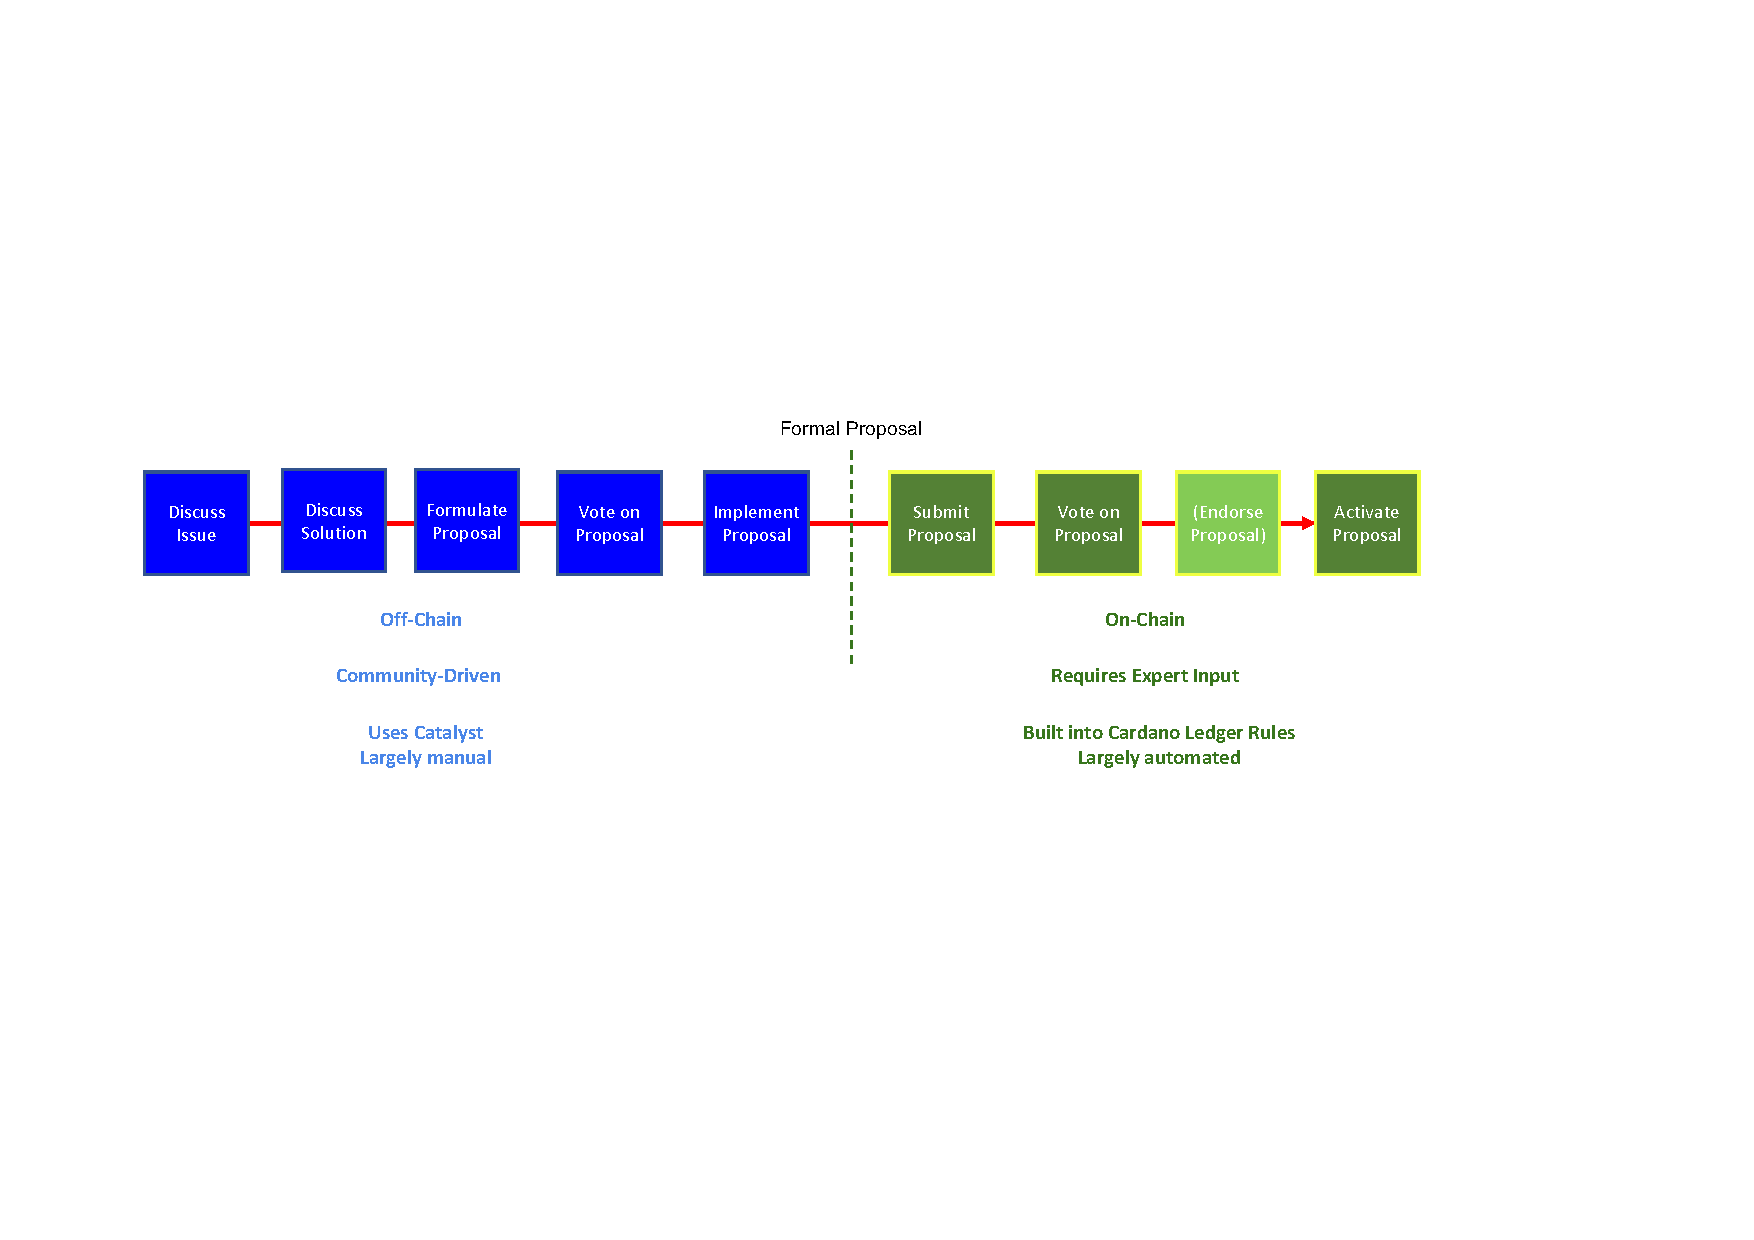
\includegraphics[trim=30 200 100 100,clip,width=\textwidth]{StoryBoard}
  \caption{Outline Process: Ideas are discussed off-chain and voted on using the Catalyst mechanism.  Successful proposals are implemented, and then submitted for on-chain voting and enactment.}
\label{fig:workflows}
\end{figure}


\newpage
\subsection{Off-Chain Process}

The off-chain process involves five key stages:

\begin{enumerate}
\item
  \textbf{Discussion.}  An issue is discussed.  This may be either formal or informal discussion, using a mechanism such as IdeaScale, a community forum such as a TeleGram channel or the Cardano Forum,
  or any other appropriate mechanism.
\item
  \textbf{Ideation.}  A concrete proposal that addresses the issue is formulated by an interested party.
\item
  \textbf{Submission.}  A proposal is submitted for voting.  The submission of proposals must follow the defined process, and may be restricted in some way.
\item
  \textbf{Voting.}  Voters may vote on whether a proposal should be progressed to implementation, requires amendment etc.  Outline or exact deadlines should be agreed as part of this process.
\item
  \textbf{Implementation.}  Accepted proposals are implemented.  For a simple proposal (eg a change to an updatable parameter), this may be as simple as capturing the intentions of the original proposal in a corresponding JSON file.
  Proposals to change protocol versions may involve significant software development, and therefore need to be funded by the Catalyst fund or some other means.
\end{enumerate}

Each of these off-chain stages may follow formally defined processes, and may be partially automated.  Generally, they will be driven by convention and rules.  A detailed governance structure is necessary to ensure that necessary business can
be transacted in an efficient and effective way, without risking loss of control to a small non-representative group, and so negating the purpose of decentralised governance.
The processes and structures may evolve over time.  Some of the issues are discussed in Appendix~\ref{sect:off-chain}.


\newpage
\subsection{On-Chain Process}

Once a proposal has been implemented in the required form, it may be submitted for enactment on-chain.  The on-chain process involves four key stages that are fully automated.  Extreme care needs to be taken with these processes,
since it may not always be possible to stop or reverse actions once they are initiated.

\begin{enumerate}
\item
  \textbf{Submission.}  A formal proposal is submitted on-chain by one of a group of submitters.  The proposal must be in the agreed format, and must include deadlines for voting, endorsement and enactment.
\item
  \textbf{Voting.}  The proposal is voted on and the votes are tallied.  If sufficient votes are obtained by the stated deadline, then the proposal is approved for enactment.
\item
  \textbf{Endorsement.}  If the proposal involves a change to the protocol, then stake pool operators must upgrade their nodes to the correct version.  This will signal their readiness to run the new protocol.
  Assuming that sufficient endorsement is obtained by the deadline, then the proposal is endorsed for enactment.
\item
  \textbf{Enactment.}  Proposals that have been approved (and endorsed, if necessary) are processed fully automatically at the corresponding epoch boundary.
\end{enumerate}

\newpage
\subsection{Key Stakeholder Groups}

A number of stakeholder groups are involved in the governance process.  The key ones are:

\begin{itemize}
\item
  \textbf{Normal Ada Holders:}
  Normal Ada holders are invested in the Cardano ecosystem in financial and other ways.
   In order to ensure fully decentralised governance, the goal of the PUP design is that normal Ada holders should have the ultimate governance power. They may, however, choose to delegate this to specialists when dealing with more technical issues, for example.
%  This ensures fully decentralised governance.
  \item
  \textbf{Stake Pool Operators:}
  Stake pool operators have the responsibility for maintaining the Cardano network.  They are heavily invested in the Cardano ecosystem through the commitment of their time, money and other resources.
  In addition to other voting rights, they need to maintain software compatibility with the latest version of the Cardano blockchain protocol.
  \item
  \textbf{End-Users:}
  These are individuals or organisations who use the Cardano blockchain to process transactions etc.  They may hold minimal ada, perhaps only on a transient basis.
  This will give them limited or no governance rights.  Their needs should, however, be considered when changes are made to protocol parameters.
  \item
  \textbf{Exchanges and other Proxy Ada Holders:}
  Exchanges and similar organisations hold Ada on behalf of other parties.  It is important from both a regulatory and a technical perspective that they do not hold excessive
  power, since this will work against the requirements of decentralisation.  They require a safe, secure and robust blockchain so that they may operate successfully on
  behalf of their clients.
\end{itemize}

The network should be able to evolve in a way that meets the best long-term needs of all these stakeholders, while maintaining the integrity, stability and longevity of
the Cardano blockchain.

\section{Detailed Design Goals}
\label{sect:goals}

The primary goals of this design are:

\begin{itemize}
\item
  \textbf{Decentralised Governance:}
  Support a decentralised governance mechanism for Cardano.
\item
  \textbf{Genesis Key Retirement:}
  Remove the dependence of the Cardano blockchain on a small set of genesis keys/delegates.
\item
  \textbf{Security:}
  Maintain the security of the Cardano network.
\item
  \textbf{Progress:}
  Ensure that the blockchain protocol can evolve in the necessary way.
\item
  \textbf{Smooth Transition:}
  Evolve smoothly from the current federated governance
\end{itemize}

Where these goals conflict, it is, of course, absolutely essential to maintain the security of the network.  Maintaining progress/enabling
evolution is also important, since otherwise governance decisions will be ineffectual/not enacted.

\pagebreak
\subsection{Overall Governance Goals}

The primary reason for decentralisation is to ensure long-term compliance with emergent and evolving international financial regulations.
Secondary reasons include improved community engagement, alignment of decision-making authority with increased responsibility for maintaining the blockchain,
ensuring the long term stability of the Cardano blockchain.  Decentralisation means that decisions about the operation and evolution of the blockchain
should be taken collectively by representive groups of stakeholders.
%
Achieving these goals requires that:

\begin{itemize}
\item
  The governance process is transparent -- the progress of decisions can be monitored and any deviations are properly explained to stakeholders.
\item
  All opinions are considered.
\item
  Control of the blockchain rests with those who have the greatest direct stake in the operation of the blockchain either as holders of ada or as maintainers of the blockchain.
\item
  Control of the blockchain is not unduly concentrated -- small, unrepresentative groups of powerful individuals should not be able to take over the operation
  of the blockchain.
\item
  The blockchain is robust to change -- it should be possible to recover from an incorrect governance decision, and any changes that are implemented will not expose the blockchain to attack.
\item
  The mechanisms that are implemented will properly incentivise stakeholders to take decisions that are in the best long-term interest of the blockchain, as well as in their own long-term interest.
\item
  There are checks and balances to ensure that technical knowledge and advice is properly considered as part of the decision making and implementation process.
  This is especially important where there are security concerns.
\item
  There is traceable continuity in the blockchain -- that is, there is an on-chain record of all the changes that are made, including the outcomes of on-chain voting, endorsement, and proposal enactment.
\item
  The transitional path to decentralised governance is clearly identified and explained, with clear steps and gates to achieving the required level of decentralisation.
\end{itemize}


It is, of course, not necessary (or probably even sensible) for every aspect of
the process to be \emph{fully decentralised}, only that
\begin{inparaenum}
\item
  the ultimate \emph{control} of
the blockchain is decentralised to the extent that is required for effective
governance, and
\item
  decentralised governance decisions are \emph{enacted} faithfully and in the
  long-term interest of the blockchain.
\end{inparaenum}
In particular, the process must not exclude those who
are less technically expert, but must properly consider technical concerns.

\subsection{Off-Chain Requirements}

There are many legitimate ways to meet the off-chain governance requirements. Appendix~\ref{sect:off-chain} considers some of the issues
that are involved.  Since this document focuses primarily on the on-chain technical design requirements, off-chain requirements will not be covered
in detail here.

\pagebreak
\subsection{On-Chain Requirements}

On-chain requirements may be split into mandatory and optional requirements.

\paragraph{Mandatory Requirements.}  The on-chain mechanism must:

\begin{itemize}
\item
  allow changes to be made to any updatable protocol parameter, in any legal way;
\item
  allow major/minor protocol versions to be upgraded;
\item
  allow the fulfilment of all kinds of central funds transfers;
\item
  not require the use of genesis keys or genesis key delegates in any part of the protocol;
\item
  allow separate per-proposal deadlines to be set for voting and endorsement;
\item
  ensure that deadlines are reasonable;
\item
  allow an epoch to be chosen for enactment of a proposal;
% \item
%   be able to faithfully enact the governance decisions that have been taken off-chain.
\item
  be secure;
\item
  be efficient;
\item
  meet the Cardano blockchain stability window requirements;
\item
  allow delegation of voting rights from ada holders to a dedicated group;
\item
  assign voting and endorsement rights in proportion to the amount of ada that is controlled;
\item
  where the proposal changes the protocol version, check that sufficient stake pools have upgraded to a compatible software version;
\item
  prevent denial-of-service attacks by limiting the proposal submission rate;
\item
  automatically enact proposals at the stated epoch boundary, provided that the necessary voting and endorsement thresholds have both been met.
\end{itemize}

\paragraph{Optional Requirements.}  In addition, the on-chain mechanism should:

\begin{itemize}
\item
  allow multiple proposals to be in-flight and enacted in a single epoch;
\item
  resolve conflicts between proposals automatically (e.g. using temporal ordering, or some other consistent and predictable mechanism);
\item
  (perhaps, allow different thresholds to be set for different kinds of proposal);
\item
  as far as possible, be consistent with the existing manual update and MIR mechanisms.
\end{itemize}

\newpage
\section{Proposal Submission}
\label{sect:submission}

Proposals are submitted by a member of a submitter group.  They must be counter-signed by a quorum of submitter keys, where the quorum is specified by the \texttt{ProposalQuorum} parameter.
%\khcomment{Difficult question: who controls registration/de-registration of submitter keys.}\pkcomment{How about an on-chain vote by ada holders?}\khcomment{That isn't possible without extending the design, of course...  You could include this as an update proposal, of course, but who submits the proposal and how do you avoid the submitter group then vetoing changes?}\khcomment{How do we
%ensure that there are always enough submitters in existence.}\pkcomment{We should have an option to reboot this set by a vote from ada holders, in case there are not enough (active) submitters}\khcomment{The
%quorum may be a protocol parameter.}\pkcomment{with an enforced sensible range in $(0,1)$}\khcomment{Yes.  I was expecting an integer value, though.  Consider the edge case where there are only a few submitters, or awkward cases where the number of submitters changes. Do you round up or down?}  No fee is charged for proposal
%submission.\khcomment{This may need to be discussed.}
A submitter may submit any number of proposals in a single epoch.
%\khcomment{This assumes that submitters are trustworthy and will not collectively spam the blockchain.  One possible solution is to use percentage of voting stake to choose the composition of this group as a subset of the delegator group.  Doing so removes one balance in the system, however (delegates propose the business that they will vote on, so potentially creating a power bloc).}
%\pkcomment{Depending on how we accumulate the counter signatures (including all of them in the transaction with the proposal, which requires off chain coordination between the submitters, or collecting them in susequent transactions) it might also be possible for a single submitter to spam the chain}
%\khcomment{The obvious approach is to use multi-sig transactions, or similar.  That would prevent multiple proposals from spamming the chain [you might be able to resubmit the same proposal, of course].  Requiring multiple transactions would be more problematic.}
It is assumed that the submitter group acts honestly on behalf of the stakeholders, and will not act to ``spam'' the chain with proposals or to prevent progress.  Suitable governance mechanisms must also be put in place to ensure that it is not possible for an unrepresentative ``cabal'' to gain control of the blockchain.

\subsection{Format}

Each proposal has a header and a body.  % and must be signed\khcomment{Submitting may implicitly sign the proposal?}.

\paragraph{Header.} The header must include:

\begin{verbatim}
"header": {
  "linked"           : ProposalHash,
  "voteby"           : Slot,
  "votethreshold"    : Threshold,
  "endorseby"        : Optional Slot,
  "endorsethreshold" : Optional Threshold,
  "enact"            : Epoch,
  "submitter"        : KeyHash
}
\end{verbatim}% \pkcomment{Do we need \texttt{Slot}, or \texttt{Epoch}?}\khcomment{You want Slot, because that is what matters for consistent voting [I assume you want the current speed of enactment]}

The \texttt{linked} field allows the proposal to be linked with the previous off-chain or on-chain acceptance (see Appendix~\ref{sect:relating-off-and-on-chain} and Section~\ref{sect:proposalid}), so enabling a chain of approval.  The \texttt{voteby} and \texttt{endorseby} fields specify deadlines.
Votes and endorsements must be received prior to the specified slot if they are to be counted.  The endorsement deadline is only required for protocol version upgrades.
%\khcomment{Arguably, to avoid performance issues, tallying should either happen at epoch boundaries or in a separate thread.}\pkcomment{Yes, same as for calculating the stake distribution and the rewards}
To avoid performance issues, tallying must be spread over time, eg in a separate thread or using a ``pulsing'' calculation. % \pkcomment{Yes, same as for calculating the stake distribution and the rewards}
In order to avoid zombie proposals that could disrupt operations, deadlines must be set within a reasonable time period after submission (e.g. within 3 epochs).
Voting and endorsement slots and thresholds are completely independent, so a voting deadline may be set before/after/at the same time as an endorsement deadline.
Deadlines can never be set in the past.
The deadline for proposal enactment must be later than the  voting and endorsement deadlines, and account for required stability windows.
%
The \texttt{votethreshold} and \texttt{endorsethreshold} fields allow specific thresholds to be set for voting and endorsement, respectively.  This allows the type of proposal to be differentiated on a per-proposal basis
(e.g. a protocol version upgrade may require a higher vote threshold than a simple parameter change)
\footnote{Arguably, this is dangerous and standard or minimum thresholds should be set as protocol parameters.}.
%
The \texttt{enact} field specifies when the proposal is to be enacted if it is approved and endorsed.  This will always be in the future.
%
The proposal submitter must belong to the correct submitter group.  \footnote{It would be possible to support
  different groups for each kind of proposal.}

The body of the proposal is specific to the proposal type.

% \newpage
\paragraph{Parameter Update Body.}  The proposal format is identical to that used for Shelley/Allegra/Mary/Alonzo. \TODO{Check the concrete format.}  Multiple parameters may be changed in a single proposal if required.
All parameters in a proposal must comply with \emph{validity} rules both on submission and on enactment.
% Parameters are checked for validity on enactment, rather than on submission, so it is possible to submit a proposal that will change parameters following a future protocol version upgrade, for example.
% \khcomment{Consider this carefully. We do need to allow initial parameters to be set.}


\begin{verbatim}
"body": {
  "parameter n" : "new value 1",
  ...
  "parameter n" : "new value n"
}
\end{verbatim}

\paragraph{Protocol Version Upgrade Body.}  The format is slightly changed from that used for Shelley/Allegra/Mary/Alonzo.


\begin{verbatim}
"body": {
  "Major"       : Integer,
  "Minor"       : Integer,
  "Genesis"     : Hash,
  "CodeVersion" : [Hash]
}
\end{verbatim}

The major and minor protocol version numbers identify the new protocol.  The genesis parameter hashes the genesis file, so ensuring that consistent initial protocol parameters are used.
The proposal also includes a list of hashes that can be used to identify one or more reference versions of the node software that implement the new protocol (e.g. as references to a specific git commit).
Node operators are not required to use one of these versions -- any software that follows the protocol rules may be be used
\footnote{Recommended software versions could also be included in the genesis file if desired.}.
% Node software only needs to comply with the new protocol rules.  It does not need to be a specific version, for example, and we do not check a software hash.
% \khcomment{I assume that
The initial set of protocol parameters is encoded in the genesis hash.

% \khcomment{We might also need to include some hash here that can be verified by the system?} % Dealt woth

\paragraph{Central Funds Transfer Body.}  The format is also identical to that used for Shelley/Allegra/Mary/Alonzo.
A single proposal may cover multiple funds transfers.  These are enacted in the order they are encountered.
% \khcomment{There is a tradeoff here: submit many proposals that may clog up the system, or submit a few.  Even if there are fewer proposals, transaction size limits mean
% that a set of transfers (for Catalyst funds, for instance), may  need to broken down into a large number of submission.}

\begin{verbatim}
"body": {
  "from"      : "Treasury"/"Reserves",
  "to"        : Optional "Treasury"/"Reserves",
  "toAddress" : Optional Address,
  "amount"    : Nat
}
\end{verbatim}

Funds may be transferred from either the treasury or the reserves, and sent to either an address, or to the treasury/reserves.
Transfers from treasury to treasury or from reserves to reserves are not permitted.  All transfers must be for a positive amount (including zero, which might be required for accounting or automation reasons). %\pkcomment{Why do we want to allow zero here?})\khcomment{I was assuming that this might be needed for accounting or automation reasons}.
Multiple transfers may be made in a single epoch.  This allows for proper accounting, where e.g. different kinds of transfer must
be authorised by different groups.

Errors in transfers between reserves and treasury, or vice-versa, may be corrected by constructing a reverse transfer that cancels the original error.
This cannot happen for transfers to addresses.  Any errors in such transfers, must be corrected by the owner of the address, who must either explicitly transfer
the funds to reserves or treasury, or else transfer the funds to a holding account\footnote{Note that there is currently no way to transfer funds back to treasury/reserves.}
Note that ledger rules ensure that the treasury and reserves may never decrease below zero (even temporarily), so that a ``double-spending attack'' is not possible.
% \khcomment{Jared to confirm.}

\subsection{Proposal Signing}

All proposals must be signed when they are submitted.  A proposal must be counter-signed by a quorum of signatures using a signing
policy that conforms to the existing \emph{multi-sig} transaction mechanism.  This enables the use of standard transaction witnessing.
% where the quorum is a protocol parameter
The signing policy is then provided as an updatable protocol parameter.  This gives a great deal of flexibility to define and change submission policies.
To reduce the possibility of abuse, the policy must comply with a minimum quorum size, which must be hard-wired into the protocol as a non-updatable
parameter.
Note that limits on transaction size will limit the maximum quorum size (currently to around 500 signatories).


%\khcomment{The obvious approach is to use transaction witnessing and a multi-sig approach, as described here.  That implies a change to the submission process, and also that
%  the submitter group is sufficiently small to allow this (I think we calculated n+m=500, where n is the actual number and m is the required number?}
% \khcomment{Using multi-sig potentially allows policies to be defined as described above.  This simplifies the system by removing the need for a separate Elector group,
%  but is perhaps open to abuse of power?}

Note that the process described here intrinsically supports automation.  Signatories can be automated agents if desired rather than individuals.  This also allows integration into a full on-chain voting mechanism in the longer term, e.g. by adopting the PriviLedge mechanisms.  The outcome of an off-chain or on-chain vote may be to construct a signed on-chain proposal for subsequent enactment.  Ultimately, if the process is purely on-chain, then the vote outcome could be embedded as the authorisation for the proposal submission without needing to construct or maintain special submitter keys.  This would improve some aspects of security, but would mean that either: i) a proposal would need to be formalised prior to the initial voting round (which might be impractical for e.g. protocol upgrades or some forms of funds transfers); or else ii) delegates would need to confirm that the proposal that was enacted was equivalent to the one that was originally agreed.


\subsection{Proposal Identifiers}
\label{sect:proposalid}

Each proposal has a unique identifier that is used for voting, endorsement, and enactment.  It may also be used to refer to the proposal in the off-chain process (eg to provide its
status, encourage voting, etc).  At a minimum, uniqueness must be enforced between submission and enactment, but it will be simplest to have full uniqueness, since the blockchain will need to record
details of each proposal indefinitely.

There are three obvious ways to construct an identifier.

\begin{description}
\item
  [Option 1.]
  An explicit identifier that is included in the proposal submission.  This could be tied, if desired, directly to the off-chain proposal/discussion.
  Care needs to be taken to ensure uniqueness of any manually assigned proposal identifier.  This is shown above as the \texttt{proposal} field.
\item
  [Option 2.]
  The identifier is constructed by hashing the submitted proposal.  This allows proposals to be identified before submission as well as during voting and enactment.  This property may be
  useful to connect off-chain and on-chain mechanisms for example.  \emph{Collision resistance} is required for the hash. % \khcomment{Confirm this.}  Confirmed.
\item
  [Option 3.]
  The transaction identifier is used to identify the proposal.  This has the advantage that it is already available on-chain, and is guaranteed to be unique.  However, it cannot be
  referred to prior to on-chain proposal submission.  Moreover, the transaction identifier cannot be relied on until the chain is stable, potentially creating confusion/an opportunity for attack.  \emph{Security cincerns therefore rule this option out.}
\end{description}

It is proposed to use Option 2, but to also include an explicit reference.  This allows
the formal proposal to be linked to off-chain or on-chain discussions and/or votes.
The reference does necessarily not need to be unique -- a single discussion or outline vote could
lead to multiple on-chain proposals.

\subsection{Proposal Validity Rules}
\label{sect:validity}

A proposal is checked for validity at two points:
\begin{enumerate}
\item
  on submission;
\item
  on enactment.
\end{enumerate}

Invalid proposals are immediately rejected and never enacted.

A proposal is \emph{valid} if it satisfies all of the following conditions:

\begin{enumerate}
\item
  it is syntactically well-formed;
\item
  all parameter values are within permitted ranges (e.g. all funds transfers are positive);
\item
  it has been (counter-)signed by a sufficient quorum of signatories;
\item
  all deadlines are sufficiently far in the future, and none is too far in the future (see Section~\ref{sect:deadlines});
\item
  protocol version upgrades correctly increment the version number against the current protocol version (see Section~\ref{sect:upgrades});
\item
  all validity conditions that apply to a specific class of proposal are also met.
\end{enumerate}

\newpage
\section{Voting on Proposals (On-Chain, Delegates)}
\label{sect:voting}

Once a properly signed proposal has been submitted on-chain, delegates may vote on whether or not to accept it.  A threshold is set for each vote.
As described in Section~\ref{sect:submission}, the thresholds for each proposal are included in the formal proposal at submission time.

\subsection{Voting}

Each \emph{registered} delegate (see Section~\ref{sect:registration}) may vote either in favour or against a proposal by submitting the corresponding transaction.  They may change their vote up to the point
where the vote is tallied.  Any changes after that point in time are not considered.  If a delegate chooses not to vote on a proposal, that is considered to be
a vote against the proposal.  Votes are submitted in the form of an on-chain transaction, and may incur fees.  The transaction needs to include:

\begin{center}
\begin{tabular}{||l|p{3in}|l||}
  \hline\hline
  proposal id & The unique identifier for the proposal, derived from the submission & 32 bytes
  \\\hline
  vote intention & Yes or no & 1 byte
  \\\hline
  Delegate public key hash & Unique identifier & 32 bytes
  \\\hline
  \hline
\end{tabular}
\end{center}

This ensures that there is a public and traceable record of each delegate's actual vote.


\subsection{Stake Snapshots}

Stake snapshots are taken at the start of each epoch.  These snapshots are currently used only for block production purposes, but they will be reused here for governance purposes.
The stake snapshot that is taken at the start of an epoch will be used for all delegated votes that are tallied at the end of the epoch.
The same stake snapshot that is used for block production is also used for endorsement.
As with block production, using fixed snapshots means that there will be a
slight delay before a change in stake will be effective for voting purposes.
However, this brings major efficiency advantages (it is not necessary to calculate specific snapshots per vote).

\begin{figure}
  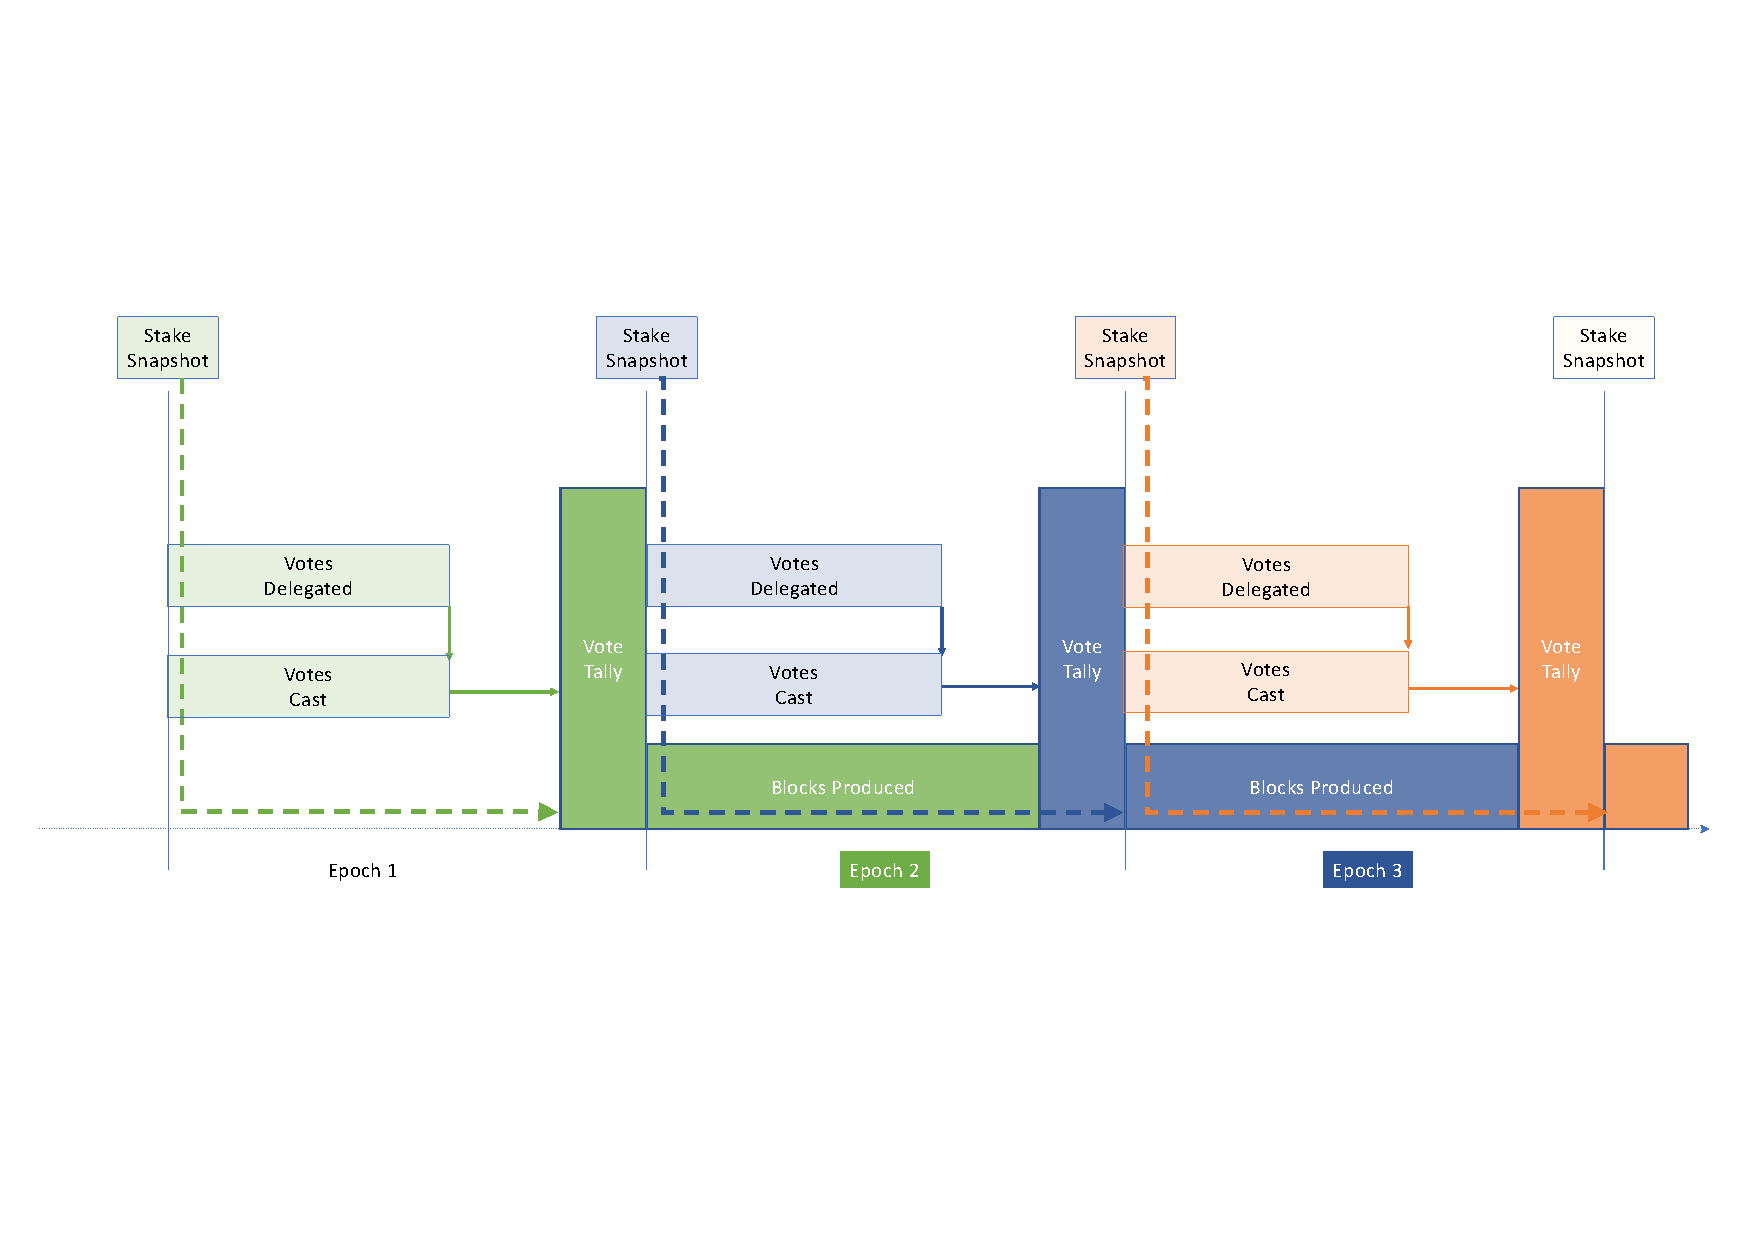
\includegraphics[trim=0 150 0 80,clip,width=\textwidth]{Stake-Snapshots}
  \caption{Stake Snapshots}
  \label{fig:stake-snapshots}
\end{figure}

Note that because of the lag in block production delegation, this design means that vote and block production stake will not be exactly aligned in an epoch.
%\khcomment{It seems sensible to separate the vote and block production snapshots like this, but it does give a slightly odd effect, in that vote and block production stake
%  will not always be the same in a given epoch.  They could be aligned, but then there will be a lag in the vote.}

 

\subsection{Tallying Votes}

Votes are tailied according to a snapshot of delegated vote that is taken at the specific point given in the proposal submission.  The stake snapshot from the start of the epoch is used to determine
the weight of each delegated vote for all votes that are tallied at the end of the epoch.  The total vote that is controlled by each delegate is the sum of all active delegations at the point that
the vote is tallied.  A calculation is made for the total amount of stake that is: i) explicitly in favour and; ii) explicitly against the proposal.  This is compared against the required voting thresholds and
if sufficient votes have been achieved, then the proposal will be accepted as decscibed below.
The tally needs to be recorded on chain.
%\khcomment{Does the tally need to be recorded on chain?}

\subsection{Voting Outcomes and Thresholds}

Following the tally, a proposal may be either accepted or rejected, based on whether it has achieved the required voting threshold.  Any proposal that achieves at least
the specified percentage of votes is accepted, and passed forward for future enactment.
The threshold for accepting a specific vote is specified in the proposal.
This must be no less than any relevant minima that are set in the protocol parameters for the specific type of proposal.
% \khcomment{there may also be minima that are set in the protocol parameters.}.
All thresholds are specified as a percentage of total ada.  There are a number of ways that this total can be specified.  In roughly declining order of size, these include:

\begin{enumerate}
\item
  The total ada that is in existence (i.e. 45 billion ada).
\item
  The total ada that is in circulation (i.e. that is not accounted in either the treasury or reserves pots) (Preferred).
\item
  The total ada that has been delegated for block production purposes in the current epoch (Preferred).
\item
  The total ada that has been delegated for voting purposes in the current epoch.
\item
  The total ada that has been used to cast a vote on a specific proposal.
\end{enumerate}


A decision needs to be taken on how to determine the total that is used in a threshold calculation\footnote{It makes sense to use the same total for all votes rather than using different totals
  for different kinds of vote.}.
Using the total ada in existence (option 1) means that very high voting thresholds cannot be achieved until all ada
is in circulation, and that ada that has not been circulated will always have a negative effect on voting.
This seems undesirable.
The second option avoids this issue, but means that ``inactive'' ada will count as a vote against a proposal, which may prevent the chain from making reasonable progress.
The third option ensures that all ``active'' participants in the blockchain are considered, but could in theory give results greater than 100\% (because of lag in the
block production snapshot compared with the voting snapshot, or if vote delegation is more popular than block production delegation).
While the fourth option may seem attractive, it may result in highly unrepresentative results if insufficient stake holders choose to delegate their vote.  This would potentially allow control of the
blockchain to be circumvented at low attack cost, so creating a security vulnerability, and would also create potential instability in the blockchain.
Likewise, the fifth option would allow proposals to pass with very little positive mandate (e.g. where only 10\% of the delegate group chose to vote on a specific issue, a majority vote could be
achieved with just over 5\% of the delegated stake).
The Priviledge project has developed further metrics that could be used to set the thresholds based on e.g. the proposal type and the
impact on the system.

\subsubsection*{Low Thresholds and Explicit Negative Voting}

One option is to require both positive and negative thresholds for a vote.  This might allow lower voting thresholds.
This approach has a number of disadvantages, however:

\begin{itemize}
\item
  The thresholds could not, anyway, be lowered significantly (or perhaps at all) without permitting unrepresentative outcomes in terms of
  favourable stake -- lower thresholds could only be accepted for certain kinds of proposal -- setting thresholds below 50\% would be hazardous, for example;
\item
  Delegates who control other delegation are already socially motivated to vote.  Delegators will remove their delegation from delegates who consistently fail to vote,
  and may require explanations for any proposal where no vote is given.
\item
  It imposes a per-vote transaction cost on normal ada holders who have chosen to register as their own delegates, and this may not be sustainable for small holders.
  This then works to reduce the number of ada holders who choose to register as delegates, consequently increasing centralisation\footnote{This assumes there is no compensation or incentive to encourage voting.}
  (Conversely, normal ada holders who do register as delegates must be positively in favour of/against a proposal by paying the requisite fee -- this acts as a deliberate drag
  to ensure some conservativism/stability in the system).
\item
  It adds complication and opportunities for gaming (eg with careful setting of thresholds);
\item
  Votes are registered on chain.  It may be socially unacceptable for a normal ada holder to vote explicitly against a proposal.  This allows an individual to have a ``silent'' negative vote.
\item
  Care needs to be taken over increasing execution costs. Tallies are potentially a critical point of performance failure, and this could perhaps double
  the cost for each tally.  High tally costs could even mean that some proposals were rejected (if they were not completed by the required deadlines, for example).
\end{itemize}

\newpage
\section{Endorsement of Proposals (Endorsers, Needed only for Protocol Version Changes)}
\label{sect:endorsement}

Proposals that change either or both the major or minor protocol version number (``hard forks'') need confirmation from the block producing nodes that they are able
to deal with the new protocol.  We term this ``endorsement''.   In previous Cardano eras, endorsement has been handled manually, as a judgement call that
is made by the blockchain operators, who are in control of the genesis keys and the core block producing nodes.  As we move away from federated control and eliminate these
mechanisms, it is necessary to automate this process.  Major protocol versions will never decrease.  Minor protocol versions will always either increase or be set to zero
(with a corresponding increase in the major protocol version number).

subsection{Automating Endorsement}

Every block producing node (``stake pool'') that wishes either to continue minting
blocks or to support the distributed verification of the Cardano blockchain must upgrade its
software to a node version that is compatible with the new protocol.  So that it
can follow the blockchain from its inception (that is, from the genesis block),
the new node software must also be prepared to handle any previous version of
the protocol, that is from version 1.0 (Byron) through all intermediate versions to the current protocol version.

There are several obvious ways that could enable an \emph{endorser} to endorse a protocol version upgrade.  A decision needs
to be made on which of these to use.

\begin{description}
\item
  [Manual endorsement.]  The endorser submits a signed transaction on-chain that confirms the maximum protocol version that they are
  able to accept (or submits an endorsement transaction for a specific proposal id).
\item
  [Automatic endorsement.]  The new software submits a signed transaction on-chain that confirms the maximum protocol version that it is
  able to accept.
\item
  [Automatic endorsement by statistical count of blocks produced.]  Each block includes the protocol version that is used by the pool that minted it.  This can be used to
  estimate the percentage of stake that is controlled by upgraded pools.
\item
  [Automatic endorsement by stake.]  Each block includes the protocol version that is used by the pool that minted it.  A map is used
  to record the most recent protocol version that is being used by each pool.  The total stake that is controlled by upgraded pools can then
  be calculated at the time of endorsement using the stake snapshot.
\end{description}

% In  cases, the transaction will need to be signed by the stake pool operational key.
Automatic endorsement has the advantage that it will always record the current
status of the pools (including any downgrades).
% However, it is not obvious that a specific proposal (identified by the proposal id) could be endorsed
% automatically.
Manual endorsement allows endorsers to have better control over
the timing of their endorsement (for example, when testing a new node version)
and to endorse specific proposals rather than a protocol version (so avoiding issues if two proposals
mistakenly refer to the same protocol version).  However, some
endorsements may be missed, and consequently some upgrade proposals might not be enacted
even though nodes are actually able to handle the new protocol.
Automating endorsements by block production reduces the number of transactions that are needed (and so reduces overhead costs for pool operators),
but unless the stake snapshot is used, this will only give a statistical measure of the upgrade status (some percentage of blocks have been produced by
pools that have upgraded).
% It may be necessary to restrict the period of endorsement to the time between proposal submission and vote tallying.
% \khcomment{Are there situations where it might make sense to upgrade pre-emptively before a proposal is submitted?}

\subsection{Tallying the Endorsements}

Endorsements are tallied following the deadline that is given in the proposal.
If there is sufficient endorsement for the proposal, then it will be carried
forward for enactment.  While the endorsement deadline is technically
independent of the voting deadline, in practice it will usually be later than the
voting deadline. That is, first the vote will be taken, then pools will indicate
their readiness to proceed with the protocol version upgrade, and if both thresholds are met,
then the proposal will be enacted.

The endorsement threshold is separate from the voting threshold, and also
may be set per-proposal.  % If the endorsement threshold is met, then the proposal is passed for enactment.
In contrast to voting, the total amount of stake that has been delegated for block production purposes is used to determine this
threshold. % \khcomment{I think it makes sense to
%   use the same snapshot that is used for normal block production rather than the
%  most recent delegation snapshot, but this should be discussed.}
To avoid chain forks, the minimum threshold for endorsement must not be less than 50\%
of the block producing stake, but may need to be higher to account for statistical variation or any errors etc.
If statistical block production is used, then the threshold should be set as a percentage of the blocks that have been produced.
This threshold should be set conservatively (e.g. a minimum of 60\% of the blocks produced).

\newpage
\section{Proposal Enactment}
\label{sect:enactment}

When the stated deadline for a proposal is reached, then it is considered for enactment.  Proposals are never considered for enactment
before the deadline.  A proposal that has been accepted by passing a voting threshold (and also, for a protocol version upgrade, the
endorsement threshold) is automatically enacted.  Enactment involves each protocol parameter being updated to the new value that is specified
in the proposal.  Changes take effect at the start of the following epoch.  A protocol version upgrade can also update other parameters as part of
the proposal, and may even change the set of parameters that can be updated.

\subsection{Protocol version changes (``Hard Forks'')}

Protocol version upgrades never decrement the protocol version.  They must increment either the current major or the current minor version by one.
If the major version is incremented, then the minor version must be set to zero.
% may be set to any required value (usually this will be zero).
Software upgrades must accept all prior protocol versions (both major and minor) that have been successfully enacted.
When a protocol version proposal is enacted, then all nodes will synchronise to the new protocol version using the ``hard fork combinator''~\cite{hardfork-combinator}.
Block production and verification will continue at the start of the next epoch using the rules that are in force for the new protocol version.

\paragraph{Major version changes override minor version changes.}
Under these rules, the only possible conflict is where one or more properly approved and endorsed proposal increments the major version and another increments the
minor version in the same epoch.  In this case, the major version change will always succeed, regardless of the order in which the proposals are enacted: if the major version change is enacted first,
then any subsequent minor version change will be invalidated.  Conversely if the minor version upgrade is enacted first, then it will be overridden by the subsequent major version upgrade.

\subsection{Prioritisation of Enactment}

If multiple update proposals are to enacted within a single epoch, then they are enacted strictly in the order that they were submitted.
This creates a deterministic order that does not need to consider when proposals achieve a majority vote, for example.
It allows proposals to be completely or partially overridden without needing an explicit cancellation option.
This approach assumes, of course, that the submitter group acts honestly and in the best interest of the protocol.
The approach does not allow contingent/conditionals proposals.  If needed, this can be handled by, for example, submitting two separate proposals that are enacted
in different epochs, where the second proposal is submitted only if the first proposal succeeds.

\subsection{Central Funds Transfers (``MIRs'')}

Several proposals for funds transfers may be enacted in a single epoch.  These proposals are enacted the in the order that they were submitted, with all ledger and
accounting rules in force.  In particular, it is not possible for the treasury, reserves or any private address to even temporarily have a negative balance.  This may affect
the ordering of transfers in some edge cases.


\addcontentsline{toc}{section}{References}
\bibliographystyle{plainnat}
\bibliography{references}

% \begin{appendix}
% \end{appendix}

\end{document}
